\documentclass{article}
\usepackage{geometry}
\usepackage{graphicx}
\title{Intelligent Security Systems\\Project - Intrusion Detection System}
\author{Sameera Desai, Appurv Jain, Sagar Parab}


\begin{document}
\maketitle
\paragraph{Executive Summary:\\}
As the technology is ameliorating, the number of hacking and intrusions are augmenting. The motive behind the attack can be personal or professional. Intrusion Detection Systems are like alarms that alerts the user of the attack. Intrusion Detection Systems monitors the networks or the system behaviors for malicious activities or behaviors. It generates reports based on these activities. They detect unauthorized accesses.\\

We will be implementing the Intrusion Detection System using R, a popular scripting language for statistical computing. R is open source and provides us with the flexibility and potency of a scripting language and has many freely available packages that implement many artificial intelligence and machine learning algorithms, statistical modeling techniques and various other useful tools. Being a scripting language, R enables us to write our own rules for misuse detection and can implement artificial neural networks using the Neural Networks package. Additionally, R provides a lot of functionality for data manipulation and visualization, which will enable us to clean and prepare the data for analysis.
	
	
\paragraph{Specification:\\}
Our decision to select R as our tool of choice was preceded by a significant amount of research on popular Intrusion detection systems such as Snort, Bro, etc. However, those tools inhibit flexibility in terms of the techniques used for anomaly and misuse detection. Additionally, snort requires constant update of rules and may not always have the updated set of rules. This is an even bigger issue now since one needs a paid subscription in order to have the latest rules.\\

Alternatively, we could have decided to use a data mining tool such as Weka, but the GUI interface is not as flexible and powerful as a scripting language. This makes it hard to do preprocess data which means we would we would either have to do it manually or use another scripting language. Therefore we decided to use R since it gives us the ability to write code that manipulates data for us.\\
 
R is an open source language for statical computation and graphics. It has a large support community and a large library of mathematical and graphical packages. Thus, R is very powerful tool and a very attractive option.\\

Some of the advantages of building an IDS using R are :
\begin{itemize}
  \item Since R is written in C and Fortran, it is very fast. This is a strong positive since many techniques used in misuse and anomaly detection are computations intensive
  \item R is open source
  \item R programs can be developed as a command line utility or have a GUI
  \item R contains a vast collection of packages that support a wide variety of data processing and modeling techniques.
  \item Hence all the tools and abilities required to build an efficient Intrusion Detection System is present in R itself
\end{itemize}
   
  
\paragraph{Methods and Techniques:\\}

In order to prepare the data for the next phase, we compiled the various data sets into two distinct data sets, one for Misuse Detection and the other for Anomaly Detection.\\

The data set for anomaly detection will contain normal usage classified as 'normal' and all the attacks, regardless of type will be classified as 'attack'. This helps us classify any pattern other than normal behavior as an attack.\\

For misuse detection, we used the 'normal' classification for normal usage and named the other attacks by their specific types.\\

We used two classifiers (Support Vector Machine and J48 Trees) for anomaly and misuse detection and used R to preprocess the data into the two data sets we would be using for the detection techniques respectively. R made it possible to write a very flexible and scalable script for data preprocessing.


 
\paragraph{Implementation:\\}
For our datasets, we used 2000 samples of normal use and 200 samples each of the 5 attack cases. That number could be very easily changed and adjusted in our script.\\
The attacks we took into consideration were as follows:
\begin{enumerate}
  \item Neptune
  \item Satan
  \item Smurf
  \item PortSweep
  \item Nmap
\end{enumerate}
We converted the given files to csv so that they were compatible with read functions in R. Then using R, we then added columns according to the attack type and then combined the various tables to form our master datasets for anomaly and misuse detection.We configured our R-script to pick random samples from the provided datasets to avoid any bias. The data sets were split into training and test for training and testing the classifiers respectively.\\
We then ran two classification algorithms on the data. We classified the data using Support Vector Machine in R using the Radial Basis kernel method which uses a Gaussian function. We also used J48 tree in Weka for additional analysis, using our preprocessed datasets as input.

 
  

\paragraph{Result:\\}
The performance of both classification methods was very strong with the lowest accuracy value significantly above 95\%. We observed that the performance of the classifiers in case of anomaly detection was slightly better that in case of misuse detection. This can be attributed to the fact that there were lesser classification levels in case of anomaly detection. Additionally, the performance of the J48 tree was observed to be slightly better than that of Support Vector Machine. Snapshots of the outputs showing confusion matrices, accuracy and some other factors are shown below. \\


\begin{figure}
  \begin{center}
    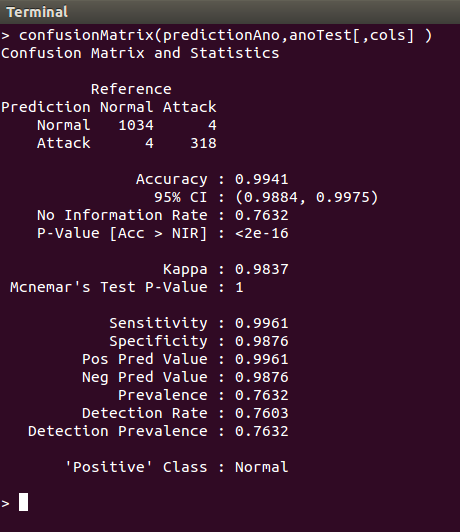
\includegraphics[scale=0.8]{Anomaly_SVM_cropped.png}
    \label{Anomaly Detection Using SVM}
    \caption{Anomaly Detection Using SVM}
  \end{center}
\end{figure}
%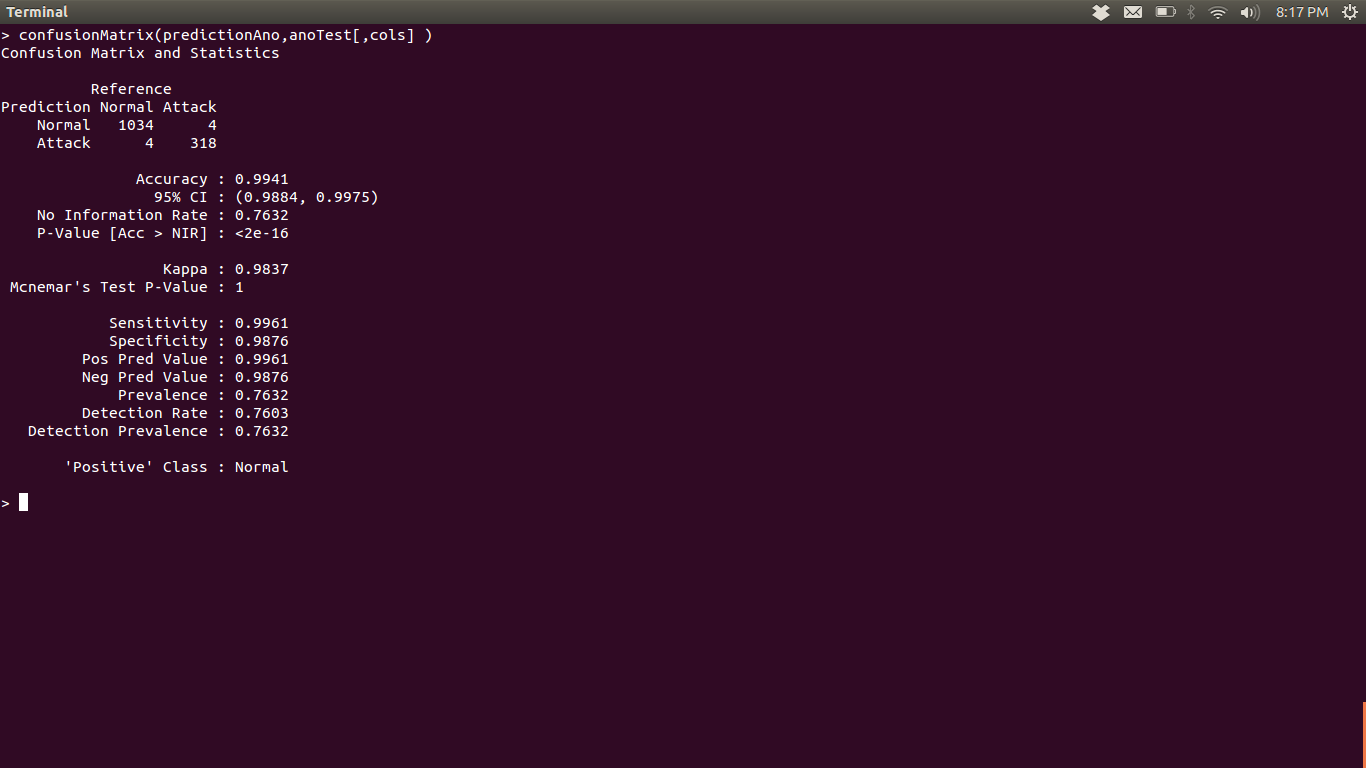
\includegraphics{Anomaly_SVM.png}


\begin{figure}
  \begin{center}
    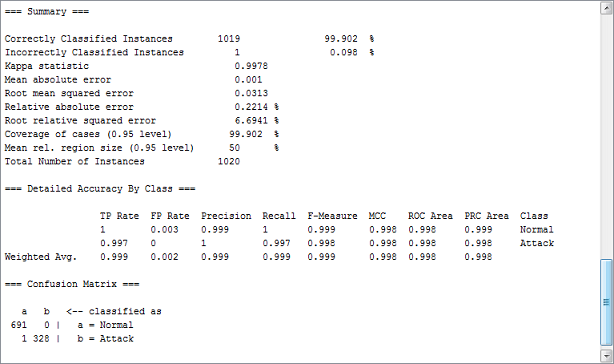
\includegraphics{Anomaly_J48_cropped.png}
    \label{Anomaly Detection Using J48 Tree}
    \caption{Anomaly Detection Using J48 Tree}
  \end{center}
\end{figure}

\begin{figure}
  \begin{center}
    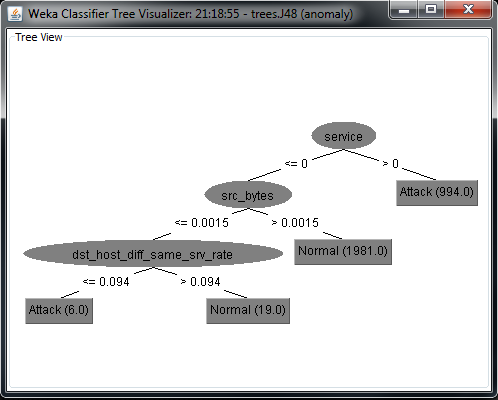
\includegraphics{Anomaly_J48_Tree.png}
    \label{J48 Tree (Anomaly Detection)}
    \caption{J48 Tree (Anomaly Detection)}
  \end{center}
\end{figure}

\begin{figure}
  \begin{center}
    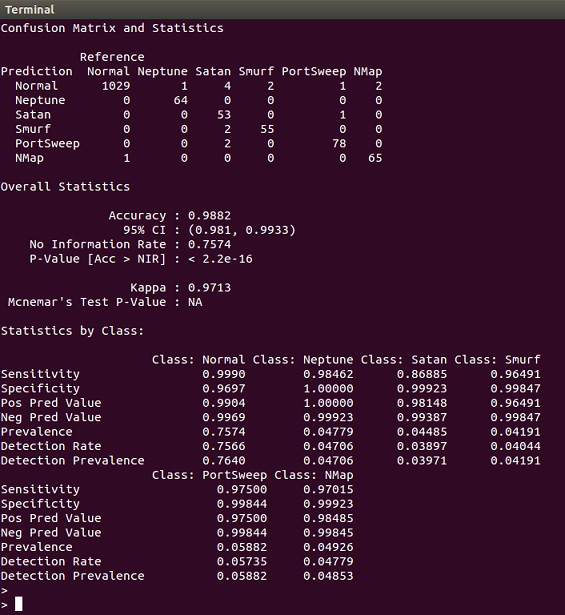
\includegraphics{Misuse_SVM_cropped.png}
    \label{Misuse Detection Using SVM}
    \caption{Misuse Detection Using SVM}
  \end{center}
\end{figure}
 
 
\begin{figure}
   \begin{center}
     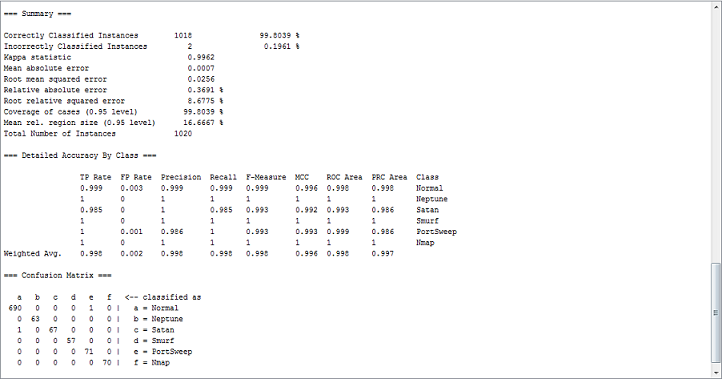
\includegraphics[scale=0.8]{Misuse_J48_cropped.png}
     \label{Misuse Detection Using J48 Tree}
     \caption{Misuse Detection Using J48 Tree}
   \end{center}
 \end{figure} 
 
 \begin{figure}
   \begin{center}
     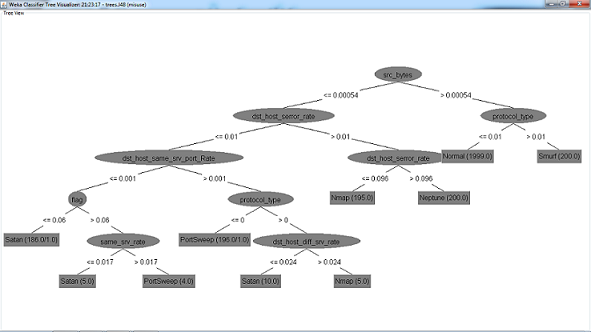
\includegraphics{Misuse_J48_Tree.png}
     \label{J48 Tree (Misuse Detection)}
     \caption{J48 Tree (Misuse Detection)}
   \end{center}
 \end{figure}
 
\end{document}
